
\begin{frame}{Turning Bands}
  \begin{itemize}
  	 \item The Turning Bands algorithm has been proposed by Matheron \cite{matheron1973intrinsic}.
    \item Turning Bands is an algorithm to transform the simulation of a Gaussian random function with covariance $C$ in $M$ simulations of independent stochastic processes with covariances $C_\theta$ (where $\theta$ is a direction and $C_\theta$ is called \textit{Spectral representation of the covariance $C$}).
    \item To generate the simulations, $M$ lines are created in different directions in a standard unit sphere in $\mathbb{R}^d$, 1D independent simulations are computed in each direction and the results are combined to generate the simulation in $\mathbb{R}^d$. 
    \item This methodology is similar to the Fourier Integral Method, where the simulation in $\mathbb{R}^d$ is transformed in the independent simulation of the angles $\theta(\omega)$ (phase simulation).
  \end{itemize}

\end{frame}

\begin{frame}{Turning Bands}
\begin{itemize}
\item Each covariance type is simulated using a specific algorithm. \cite{emery2006tbsim}
\item To simulate covariances that are result of a linear combination of basic models (spherical, exponential, Gaussian, nugget, etc...), we simulate independently each model and the results are combined.
\item Because the 1D simulation in each node is completely independent, 
we can easily parallelize the simulation in space without any synchronization technique. 
\item The Turning Bands method can be seen as a generalization of the spectral method \cite{lantuejoul2013geostatistical}. Note that we can use FIM 1D to simulate the 1D covariance models. 
\end{itemize}
\end{frame}

\begin{frame}{Turning Bands}
\begin{itemize}
 \item The relationship between the simulation of independent stochastic processes and the simulation of the original Gaussian random function is given by 
 \begin{equation}
  Y^{(n)}(x) = \frac{1}{\sqrt{n}} \sum_{k=1}^{n} X_k(<x,\theta_k>), x \in \mathbb{R}^d
 \end{equation}
 where $(\theta_n, n \in \mathbb{N})$ is a sequence of directions on an unit sphere $S_d$ and $(X_n, n \in \mathbb{N})$ is a sequence of
 independent stochastic processes with covariance $C_{\theta_n}$. $\rho_k = <x, \theta_k>$ is the projection of the vector
 $x$ in direction $\theta_k$ and $X_k(\rho_k)$ is the spectral representation of the Gaussian random function $Y^{(n)}(x)$ in
 the direction $\theta_k$.
\end{itemize}
\end{frame}

\begin{frame}{Turning Bands}
\begin{itemize}
\item The covariance $C^{(n)}(h)$ of $Y^{(n)}(x)$ is described by
\begin{equation}
C^{(n)}(h) = \frac{1}{n} \sum_{k=1}^{n} C_{\theta_k}(<h, \theta_k>)
\end{equation}

where $C_{\theta_k}(<h, \theta_k>)$ is the spectral representation of the covariance $C^{(n)}(h)$ along direction $\theta_k$.

\item If the covariance $C$ is isotropic, i.e., can be written as $C(h)=C_d(|h|)$ for some scalar function $C_d$ defined on 
$\mathbb{R}^{+}$, then the relationship between $C_1$ and $C_d$ is given by

\begin{equation}\label{eq_cov_d}
 C_d(r) = 2 \frac{(d-1)\omega_{d-1}}{d\omega_{d}} \int_{0}^{1}(1-t^2)^(\frac{d-3}{2})C_1(tr) dt
\end{equation}

where $\omega_{d}$ stands, as usual, the d-volume of the unit ball in $\mathbb{R}^d$. 
\end{itemize}
\end{frame}


\begin{frame}{Turning Bands}
 \begin{itemize}
  \item If $d=3$, the equation (\ref{eq_cov_d}) is reduced to
  \begin{equation}
    C_3(r) = \int_{0}^{1}C_1(tr)dt
  \end{equation}
  
  or equivalently
  \begin{equation}
   C_1(r) = \frac{d}{dr}rC_3(r)
  \end{equation}

  Curiously, for $d=2$ the relationship is more complicated
  \begin{equation}
   C_2(r) = \frac{1}{\pi}\int_{0}^{\pi}C_1(r sin(\theta))d\theta
  \end{equation}
  
  and
  
  \begin{equation}
   C_1(r) = 1 + r \int_{0}^{\pi/2} \frac{d}{dr}C_2(r sin \theta) d\theta
  \end{equation}


 \end{itemize}

\end{frame}

\begin{frame}{The Turning Bands algorithm} 

 Keeping in mind the previous results, the Turning Bands algorithm can be written as:
 
\begin{block}{}\label{tb.algo}
\begin{enumerate}
 \item Generate a set of directions $\theta_1, ..., \theta_n$ such that $\frac{1}{n}\sum_{k=1}^{n}\delta_{\theta_k} \approx \varpi$.
 \item Generate independent standard stochastic processes $X_1, ..., X_n$ with covariances functions $C_{\theta_1}, ..., C_{\theta_n}$.
 \item Compute $\frac{1}{\sqrt{n}}\sum_{k=1}^{n}X_k(<x, \theta_k>)$ for any $x \in D$.
\end{enumerate}
\end{block} 

In this algorithm, $D$ is the simulation domain, $\delta_{\theta_n}$ is a distribution where $\sum_{k=1}^{n}\delta_{\theta_k}$
converges weakly to $\varpi$, the uniform distribution over $S_d$ (unit sphere in $\mathbb{R}^d$). 
\end{frame}


\begin{frame}{Turning Bands: Generating the directions}
There are three main ways to generate directions $\theta_n$ satisfying the TB condition:
\begin{itemize}
 \item Arrange $\theta_n$ regularly on $S_d$. This approach is efficient in $d=2$, but for $d>2$
 this solution does not work well. In $d=3$, for example, the maximum number of regular directions is equal to 15.
 \item Generate $\theta_n$ using a uniform distribution in $S_d$ works. 
 But, using this method, the convergence of $\frac{1}{n}\sum_{k=1}^{n}\delta_{\theta_k}$
 is very slow, i.e., we need many lines to generate good results.
 \item Use a sequence with weak discrepancy \cite{freulon1994conditional}, where the directions are generated using a pseudo-random sequence of directions.
 \end{itemize}

\end{frame}


%\begin{frame}
%\frametitle{Turning Bands: Generating the directions}
%\begin{itemize}
% \item Use a sequence with weak discrepancy. For $d=3$, \cite{freulon1994conditional} propose the sequence:
% \begin{equation}
% \begin{aligned}
 % u_n = \frac{a_0}{2} + \frac{a_1}{4} + ... + \frac{a_p}{2^{p+1}} \\
%  v_n = \frac{b_0}{3} + \frac{b_1}{9} + ... + \frac{b_p}{3^{q+1}} \\
%  \theta_n = \left( \cos(2\pi u_n) \sqrt{1-v_n^2}, \sin(2\pi u_n) \sqrt{1 - v_n^2}, v_n \right)
%  \end{aligned}
% \end{equation}
 
% where $a_i = 0, 1$ and $b_j = 0, 1, 2$ and $n=a_p...a_2a_1a_0=b_q...b_2b_1b_0=a_0 + 2a_1 + ... + %2^pa_p=b_0+3b_1+...3^qb_q$. In other
% words, $a_i$ and $b_j$ are the digits of the binary and ternary representation of $n$, respectively.
%\end{itemize}
%\end{frame}

\begin{frame}{Turning Bands: Generating the directions}

The Freulon's algorithm produces $\theta_n$ as far as possible from $\theta_1, ... , \theta_{n-1}$ and fills the sphere $S_d$ as
fast as possible. As can be seen in the Figs. \ref{fig:freulon_algo_10_bands}, \ref{fig:freulon_algo_100_bands}, 
\ref{fig:freulon_algo_1000_bands}, using 1000 bands is possible to generate a dense set of points filling the sphere $S_d$. The generated sequence of directions $\theta_n$ using this algorithm is unique, but other configurations can be generated applying random band rotations on the original sequence $\theta_n$. 

In practice, Freulon's algorithm assures a fast convergence to the TB algorithm. Generally, to large datasets using 1000 or 2000 directions
it is possible to generate good results. 
\end{frame}


\begin{frame}
\frametitle{Turning Bands: Generating the directions}
\begin{figure}
\begin{center}
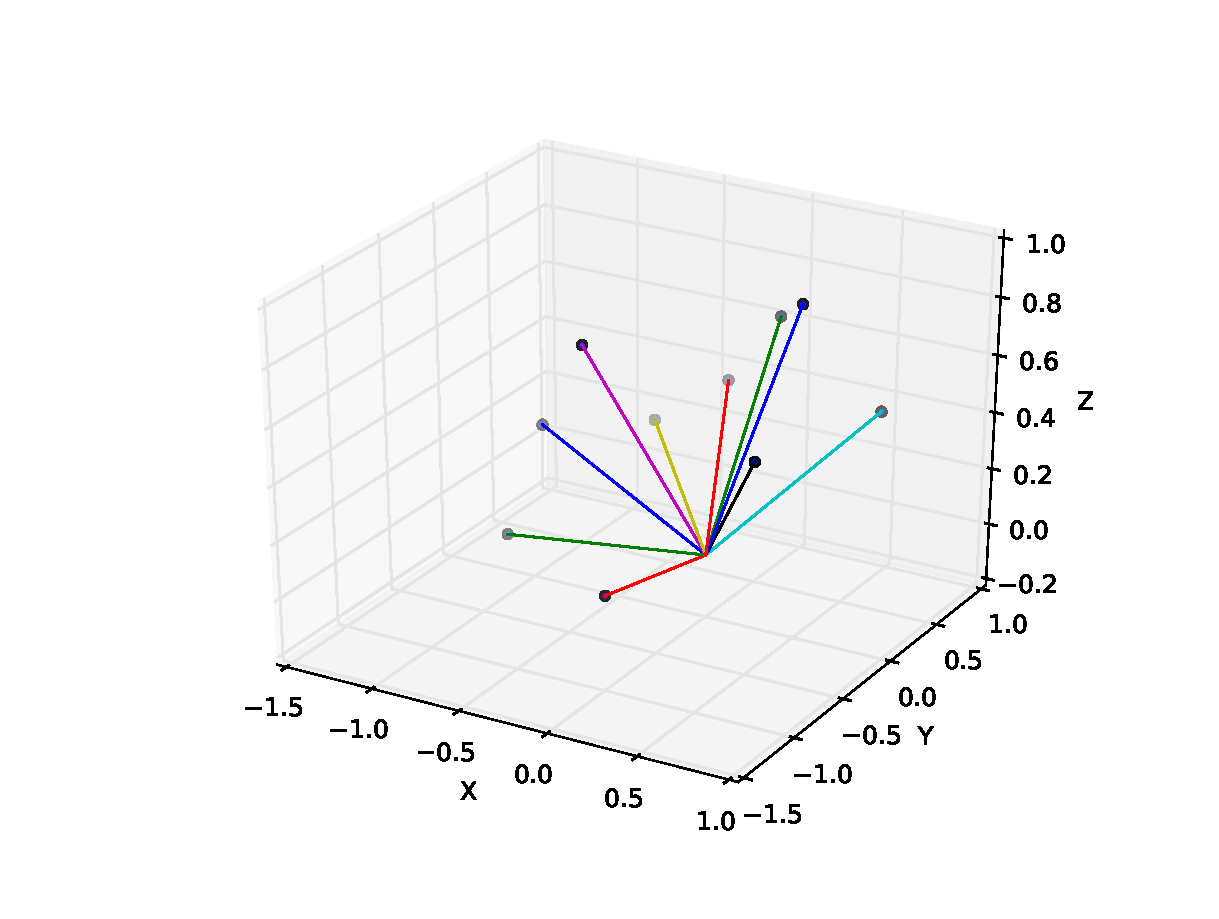
\includegraphics[height=0.7\textheight]{figs/freulon_algo_10_bands.pdf}
\end{center}
\caption{10 bands generated using the Freulon's algorithm}
\label{fig:freulon_algo_10_bands}
\end{figure}
\end{frame}


\begin{frame}
\frametitle{Turning Bands: Generating the directions}
\begin{figure}
\begin{center}
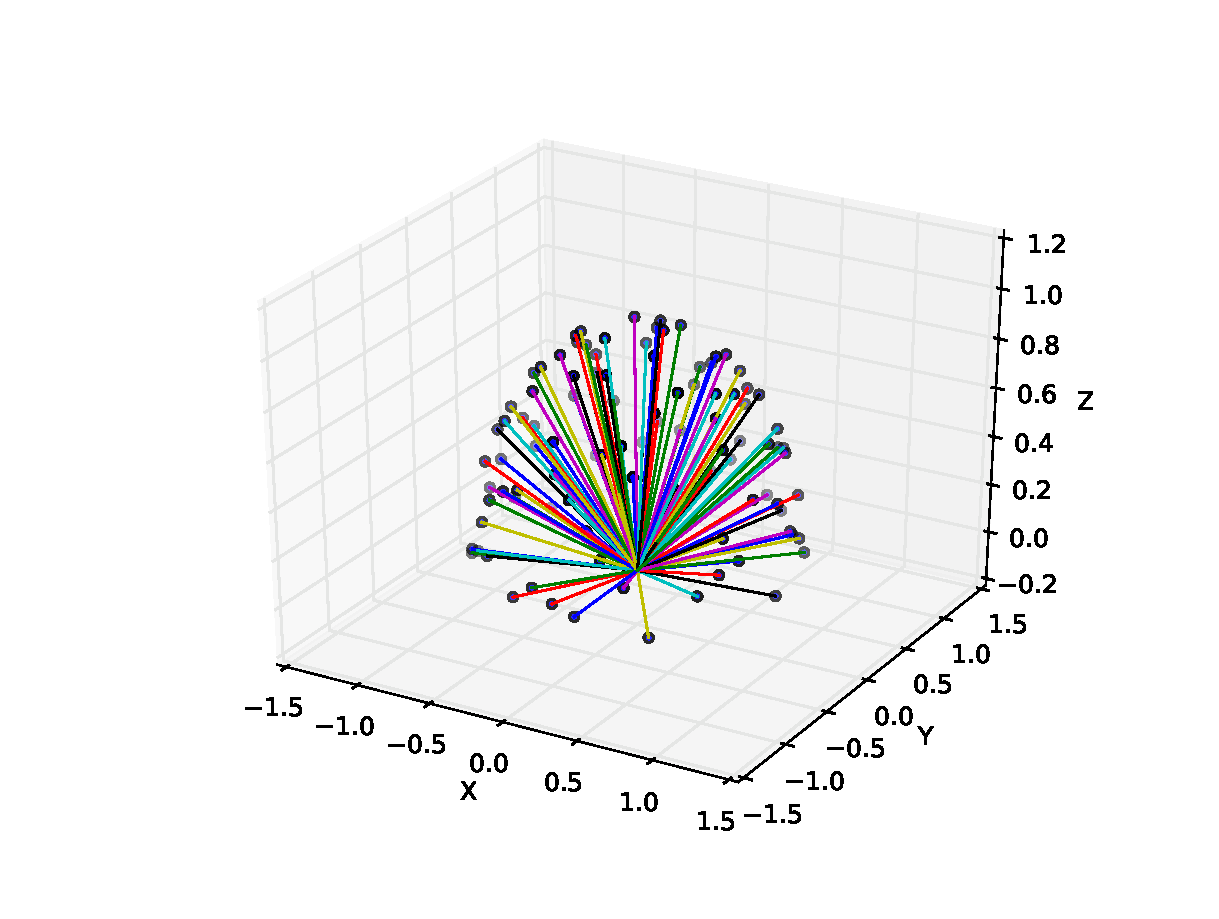
\includegraphics[height=0.7\textheight]{figs/freulon_algo_100_bands.pdf}
\end{center}
\caption{100 bands generated using the Freulon's algorithm}
\label{fig:freulon_algo_100_bands}
\end{figure}
\end{frame}


\begin{frame}
\frametitle{Turning Bands: Generating the directions}
\begin{figure}
\begin{center}
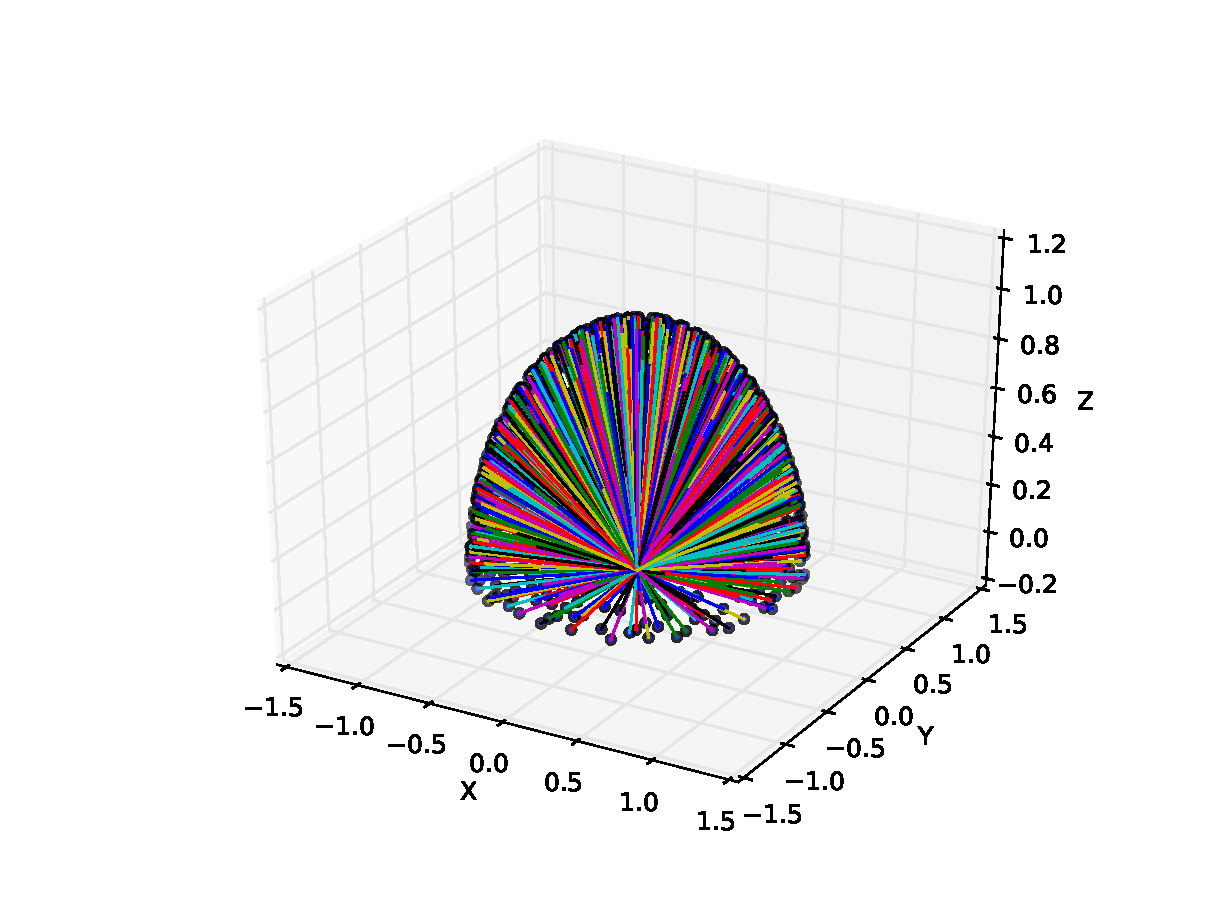
\includegraphics[height=0.7\textheight]{figs/freulon_algo_1000_bands.pdf}
\end{center}
\caption{1000 bands generated using the Freulon's algorithm}
\label{fig:freulon_algo_1000_bands}
\end{figure}
\end{frame}


\begin{frame}{Turning Bands: Generating the unidimensional simulations}
 
 Turning Bands algorithm does not determine an algorithm to generate the independent stochastic process along each band. 
 Hence, in practice, for each model and band we generate independently the stochastic process using the appropriated 
 algorithm to the specific model. After the execution of all independent simulations in a direction $\theta_n$, 
 the results are combined to generate the final result in this direction. In \cite{emery2006tbsim} is presented 15 algorithms to generate 15 different types of Covariance models.
 
\end{frame}

\begin{frame}
\frametitle{Conditioning the spectral simulations}
 In the previous slides, I presented some techniques to simulate stochastic process associated with some covariances models. Now,
 I will present the algorithm to generate the conditional simulations using Turning Bands (or other type of algorithm)
 in the simulation domain $D$. 
 In this algorithm, $CD$ stands for conditioning data-set.
 
\begin{block}{Conditional simulation of a Gaussian Random Function}
 \begin{enumerate}
  \item Simulate a Gaussian random function $y$ (using Turning Bands or other type of simulation algorithm) with mean $0$ and covariance $C$
  in  domain $D$ and at the conditioning points. Let ($y(x), x \in D$) and ($y(c), c \in CD$) be the generated values in the simulation domain and in the conditioning data-set, respectively.
  \item Calculate the kriged estimates $r(x) = \sum_c\lambda_c(x)(z(c) - y(c))$ for each $x \in D$. Let $z(c), c \in CD$ be the conditioning data. $r(x)$ is the residual value.
  \item Return $y(x) + r(x), x \in D$, the conditional simulation.
 \end{enumerate}

\end{block}

\end{frame}


\begin{frame}{Turning Bands: some observations}
 \begin{itemize}
  \item The quality (convergence velocity) of the Turning Bands is directly related to the number of lines and to the algorithm
  used to generated the band directions.
  \item In the practice, using the Freulon's algorithm, a number of lines greater than 1000 is enough to generate good results \cite{emery2006tbsim}.
  \item When the number of lines is not appropriated, artifacts are generated.
  \item The Turning Bands is a \textit{share nothing} algorithm, so it's very easy to implement a highly efficient distributed version
  of this algorithm. Ar2GeMS has a implementation using openMP.
 \end{itemize}
\end{frame}


\begin{frame}{Turning Bands: the impact of the number of bands}
 
\begin{figure}
\begin{center}
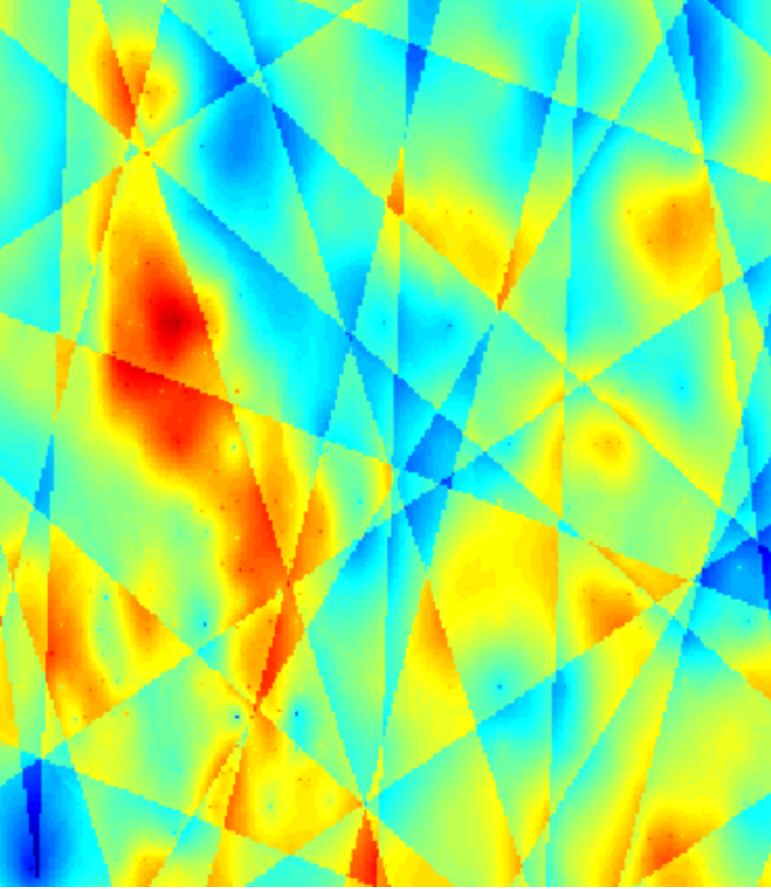
\includegraphics[width=0.5\textwidth]{figs/walker_lake_tb_n_10.pdf}
\end{center}
\caption{Conditional simulation of the Walker lake data-set with number of lines equal to 10.}
\label{fig:gaussian_unc_simulation}
\end{figure}
\end{frame}

\begin{frame}{Turning Bands: the impact of the number of bands}
\begin{figure}
\begin{center}
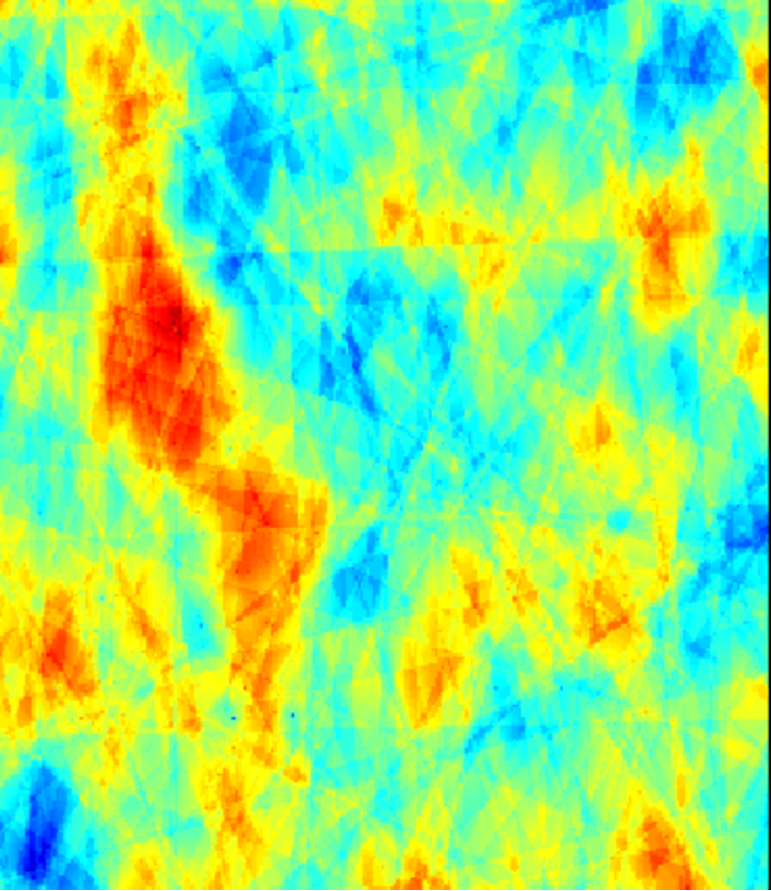
\includegraphics[width=0.5\textwidth]{figs/walker_lake_tb_n_100.pdf}
\end{center}
\caption{Conditional simulation of the Walker lake data-set with number of lines equal to 100.}
\label{fig:gaussian_unc_simulation}
\end{figure}
\end{frame}

\begin{frame}{Turning Bands: the impact of the number of bands}
\begin{figure}
\begin{center}
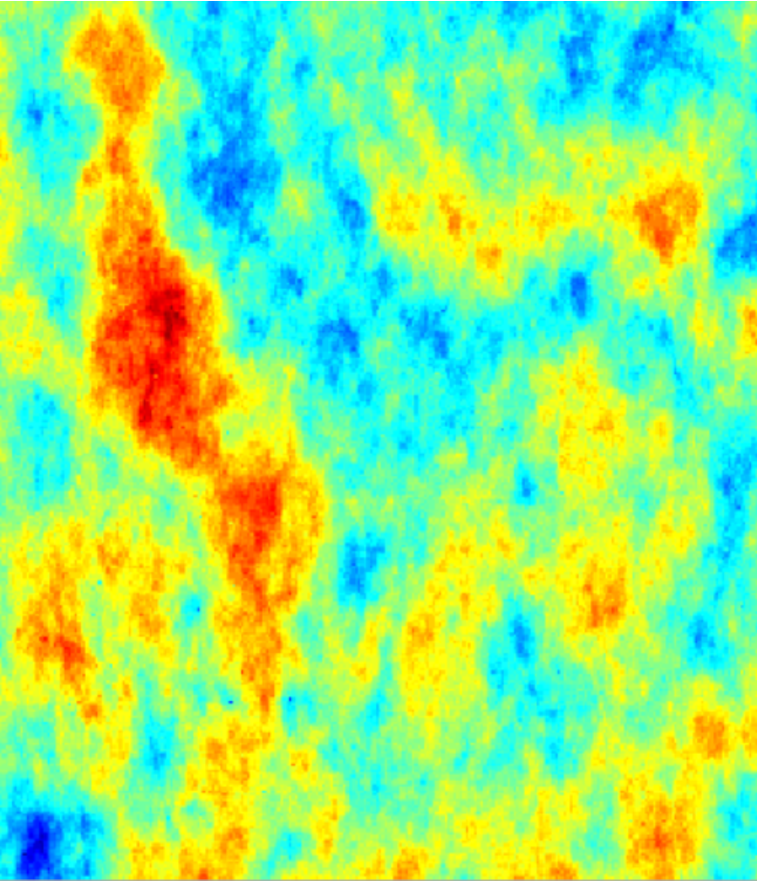
\includegraphics[width=0.5\textwidth]{figs/walker_lake_tb_n_1000.pdf}
\end{center}
\caption{Conditional simulation of the Walker lake data-set with number of lines equal to 1000.}
\label{fig:gaussian_unc_simulation}
\end{figure}
\end{frame}

